\section{Introduction}
Traditional assertions express logical properties that help programmers design and
reason about the correctness of their program. Verification tools
guarantee that every execution will satisfy an assertion, such as the
absence of null dereferences or a legal value range for a variable.
However, many applications produce or consume probabilistic data, such as the
relevance of a document to a search, the distance to the nearest
coffee shop,
or the estimated arrival time of the next bus. From smartphones with
sensors to robots to machine learning to big data to approximate
computation, many applications use probabilistic
values.

Current assertion languages and verification tools are insufficient in
this domain.  Traditional assertions do not capture probabilistic
correctness because they demand that a property hold on \emph{every}
execution.  Recent work on inference in probabilistic programming
languages builds language abstractions to aid programmers in describing
machine learning models but
does not deal with verification of probabilistic correctness
properties~\cite{infernet, church, pmonad, PPT:05}. Sankaranarayanan et al.~\cite{sriram-pldi} address the
verification of programs in probabilistic programming
languages through polyhedral volume estimation,
but this approach limits the domain to programs with linear arithmetic
over constrained probability distributions.
In contrast, this work
defines a semantics for computing in mainstream languages over a broader set of distributions
with sampling functions
but does not verify programs.

We propose \emph{probabilistic assertions}
(\passerts), which express probabilistic program properties, and
\emph{probabilistic evaluation}, which verifies them.  A \passert
statement is a probabilistic logical statement over random
variables. \emph{Probabilistic evaluation} extracts, optimizes, and
evaluates the distribution specified in a \passert by
combining techniques from static verification,
symbolic execution, and dynamic testing.

\paragraph*{Probabilistic Assertions} 
Programmers write \code{passert e, p, cf}
to check the probability that the Boolean expression \code{e} holds in
a given execution of the program is at least \code{p} with confidence
\code{cf}. The parameters \code{p} (defaults to 0.5) and \code{cf}
(defaults to 95\%) are optional. Our analysis estimates the likelihood
that \code{e} is true, bounds any error in that estimate, and determines
whether that
estimate is significantly different from
\code{p}. 
For example, consider the following function, which adds
Gaussian noise to users' true locations to protect their privacy.
%
\begin{lstlisting}
  def obfuscate_location(location):
    noise = random.gauss(0,1)
    d = distance(location, location + noise)
    passert d < 10, 0.9, 95%
    return location + noise
\end{lstlisting}
%
To ensure that obfuscation does not change a user's true location too
much, the programmer asserts that the Euclidean distance between the
true and obfuscated location should be within 10 miles at least 90\%
of the time with 95\% confidence. While occasional outliers are
acceptable, the programmer wants to ensure that the common case is
sufficiently accurate and therefore useful.

A traditional assertion---\code{assert d < 10}---does not
express this intent.  Since the Gaussian distribution has a non-zero
chance of adding any amount of noise, some executions will make
\code{d} greater than 10.  Since these infrequent outlier cases are possible,
traditional verification must conclude that the assertion does not hold.

\paragraph*{Probabilistic Evaluation} Probabilistic evaluation
verifies the probabilistic logical statement over random variables
expressed by the \passert. It first performs \emph{distribution extraction},
which is a symbolic execution that builds a Bayesian
network, a directed, acyclic graphical model. Nodes
represent random variables from the program and edges between nodes
represent conditional dependences between those random variables.
This process defines a probabilistic semantics in which \emph{all}
variables are distributions. Constants (e.g., \code{x = 3}) are
point-mass distributions.  Random distributions, both simple (uniform,
Gaussian, etc.) and programmer-defined, are represented
symbolically.  Other variables are defined in terms of these basic
distributions.

For example, let $L$,
$D$, and $N$ be the random variables corresponding to the variables
\code{location}, \code{d}, and \code{noise} in the above program.  The
\passert constrains the probability $\prob{D < 10}$ given that $L$ is
a point-mass distribution and that $N$ is drawn from a Gaussian:
%
$$ \prob{D < 10~|~L = \mathsf{location}, N \sim \mathcal{N}(0,1)} > 0.9 $$
%
This inequality constrains the probability of correctness for a particular
input location.  Alternatively, programmers may express a distribution
over expected input locations by, for example, setting the
\code{location} variable to sample from a uniform distribution. The
\passert then measures the likelihood that the obfuscation will yield
acceptable results for uniformly distributed input locations:
%
$$ \prob{D < 10~|~L \sim \mathcal{U}, N \sim \mathcal{N}(0,1)} > 0.9 $$

\begin{figure}
    \begin{center}
    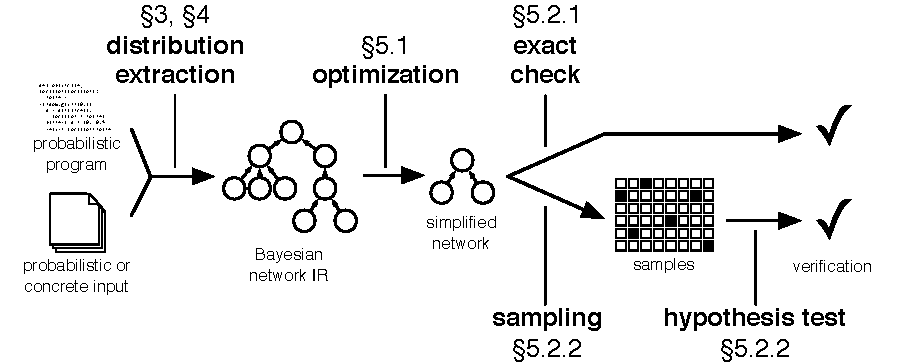
\includegraphics[width=\columnwidth]{figs/overview.pdf}
    \end{center}
    \vspace*{-1.0ex}
    \caption{\tool's workflow to verify probabilistic
    assertions.}
    \label{passert:fig:overview}
\end{figure}


Our key insight is that, with this probabilistic semantics for
\passerts, we can optimize the Bayesian network representation and
significantly improve the efficiency of verification.  Using known
statistical properties, our optimizations produce a simplified but
equivalent Bayesian network. For example, we exploit identities of
common probability distributions and Chebyshev's inequality.  In some
cases, these simplifications are sufficient to facilitate direct
computation and verify the \passert precisely. Otherwise, we sample
the simplified Bayesian network and perform a hypothesis test to
statistically verify the \passert. We use
\emph{acceptance sampling}, a form of hypothesis testing, to bound the
chance of both false positives and false negatives subject to a
confidence level.  Programmers can adjust the confidence level to
trade off between analysis time and verification accuracy.


\paragraph*{Evaluation}
We implement this approach in a tool called \tool that takes C and C++
programs with \passerts as inputs. \tool emits either \emph{true},
\emph{false}, or \emph{unverifiable} along with a confidence interval
on the assertion's probability.  Figure~\ref{passert:fig:overview} gives an
overview.  We implement the entire toolchain for \tool in the LLVM
compiler infrastructure~\cite{llvm}.  First, \tool transforms a
probabilistic C/C++ program into a Bayesian network that expresses the
program's probabilistic semantics. For program inputs, developers
provide concrete values or describe input distributions. \tool
optimizes the Bayesian-network
representation using statistical properties and then either
evaluates the network directly or performs sampling.

We implement case
studies from three application domains: sensors, data obfuscation, and
approximate computing.  We show that \passerts express their
correctness properties and that \mayhap offers an average speedup of
\perfdata{o-speedup-harmmean-sample} over stress testing with rote
sampling.
\tool's benefits over simple stress testing---repeated execution of
the original program---are threefold. First, statistical
simplifications to the Bayesian network representation reduce the work
required to compute each sample:
for example, reducing the sum of two
Gaussian distributions into a single Gaussian halves the necessary
number of samples.
Second, distribution extraction has the effect of
partially evaluating the probabilistic program to slice away the
non-probabilistic parts of the computation. Sampling the resulting
Bayesian network eliminates wasteful re-execution of deterministic
code. Third, our approach either directly evaluates the \passert or derives
a number of samples sufficient for statistical significance.
It thereby provides statistical guarantees
on the results of sampling that blind stress testing does not guarantee.

Although programs that compute with probabilistic data are already
ubiquitous, abstractions and tools to help their developers are
lagging.  By harnessing randomness, our approach introduces new and
effective abstractions for correctness, optimization, and
verification of probabilistic programs.

%%% Local Variables: 
%%% mode: latex
%%% TeX-master: "paper"
%%% End: 
